\documentclass[%
fontsize=10%
,a5paper%
,DIV=15%
]{scrartcl}
%scrartcl



\usepackage{gredocument}
\usepackage{psaume}

\title{\centrer{Veillée pascale}}
\author{la nuit de la Résurrection}
\date{avec baptêmes d'adultes}

\makeindex
\definecolor{rubrum}{rgb}{.6,0,0}
\def\rubrum{\color{rubrum}}%%%%%%%mettre"\def\rubrum{\color{rubrum}}" pour avoir le texte adéquat en rouge
\def\nigra{\color{black}}
%    \redlines
%    \definecolor{gregoriocolor}{rgb}{.6,0,0}
%
%\let\red\rubrum

\begin{document}


\maketitle

\newfontfamily\lettrines[Scale=1.3]{LettrinesPro800}
    \def\gretextformat#1{{\fontsize{\taillepolice}{\taillepolice}\selectfont #1}}
    \def\greinitialformat#1{{\lettrines #1}}

\titre{Bénédiction du feu et du cierge}
\vspace{0.5cm}
\rubrica{Le Christ, "lumière du monde" (Jn,8,12) va illuminer tout homme cette nuit en sortant du tombeau, il va dissiper les ténèbres du péché}
\rubrica{Le prête bénit le feu, puis trace sur le cierge la croix, l'alpha et l'oméga, et les chiffres de l'année}
\begin{center}
\versio{Christus Heri et hodie}{Le Christ hier et aujourd'hui}
\versio{Princ\'ipium et Finis}{Commencement et Fin}
\versio{Alpha et Omega}{Alpha et Omega}
\versio{Ips\'ius sunt témpora et s\'æcula}{A lui sont les temps et les siècles}
\versio{Ipsi glória et impérium}{A Lui gloire et domination}
\versio{per univérsa aeternit\'atis s\'æcula. Amen}{pendant tous les siècles de l'éternité. Amen}
\end{center}
%\vulgo{1. Venez, Esprit-Saint Créateur, dans les âmes de vos fidèles : comblez de la grâce d'en haut les c\oe urs que vous avez créés.}

%\cantus{Hymne}{VeniCreator}{}{}
%\noindent
\traduire{%
2.~Qui díceris Paráclitus,\\%
Altíssimi donum Dei,\\%
Fons vivus, ignis, cáritas\\%
Et spiritális únctio.}{%
2.~Vous qu'on appelle Consolateur,\\%
don du Dieu très-haut,\\%
source vive, feu, charité\\%
et onction spirituelle.\\%

}

\traduire{%
3.~Tu septifórmis múnere,\\%
Dig\textit{i}tus patérnæ déxteræ,\\%
Tu rite promíssum Patris,\\%
Sérmone ditans gúttura.}{%
3.~Vous l'Esprit aux sept dons,\\%
le doigt de Dieu,\\%
la promesse authentique du Père,\\%
qui mettez sa parole sur nos lèvres.\\%

}


\traduire{%
4.~Accénde lumen sénsibus,\\%
Infúnd\textit{e} amórem córdibus,\\%
Infírma nostri córporis\\%
Vírtute firmans pérpeti.}{%
4.~Éclairez nos esprits de votre lumière,\\%
mettez l'amour dans nos c\oe urs~;\\%
soutenez la faiblesse de notre corps\\%
par votre constante vigueur.\\%

}


\traduire{%
5.~Hostem repéllas lóngius,\\%
Pacémque dones prótinus~:\\%
Ductóre sic te pr\'ævio\\%
Vitémus omne nóxium.\\}{%
5.~Chassez l'ennemi loin de nous,\\%
donnez-nous sans retard la paix~;\\%
guidez-nous, et que sous votre conduite\\%
nous évitions tout mal.\\%
}

\traduire{%
6.~Per te sciámus da Patrem,\\%
Noscámus atque Fílium,\\%
Tequ\textit{e} utriúsque Spíritum\\%
Credámus omni témpore.\\}{%
6.~Faites-nous connaître le Père,\\%
faites-nous connaître le Fils,\\%
donnez-nous de toujours croire en vous\\%
qui êtes l'Esprit du Père et du Fils.\\%
}

\traduire{%
7.~Deo Patri sit glória,\\%
Et Fílio qu\textit{i} a mórtuis\\%
Surréxit, ac Paráclito,\\%
In sæculórum sǽcula.\\%
Amen\\}{%
7.~Gloire soit à Dieu le Père,\\%
et au Fils ressuscité des morts,\\%
et à l'Esprit consolateur\\%
dans les siècles des siècles.\\%
\ainsi\\%
}

\traduire{%
℣.~Emitte Spiritum tuum et creabúntur.}{%
℣.~Envoyez votre Esprit Seigneur et il se fera une création nouvelle.}

\traduire{\textbf{%
℟.~Et renovábis fáciem terræ.}}{\textbf{%
℟.~Et vous renouvellerez la face de la terre.}}

\traduire{%
Orémus.}{%
Prions.}

\traduire{%
Deus, qui corda fidélium Sancti Spíritus illustratióne docuísti : da nobis in eódem Spíritu recta sápere, et de eius consolatióne gaudére. \Perdominum \quitecum \peromnia%
}{%
Ô Dieu, qui avez éclairé les cœurs de vos fidèles par la lumière du Saint-Esprit, donnez-nous par ce même Esprit de comprendre et d'aimer ce qui est bien, et de jouir sans cesse de ses divines consolations. \Parjesus \quietant \siecles}
\amen




\V Le Seigneur soit avec vous.

\R \textbf{Et avec votre esprit.}

Prions\\
Jetez les yeux, Seigneur, sur ces époux vos serviteurs et protégez cette institution que vous avez établie pour la propagation du genre humain, afin qu'unis par vous ils soient également soutenus et gardés par votre secours. Par le Christ Notre-Seigneur.

\R \textbf{Ainsi soit-il.}
\vspace*{3cm}
%\begin{center}
%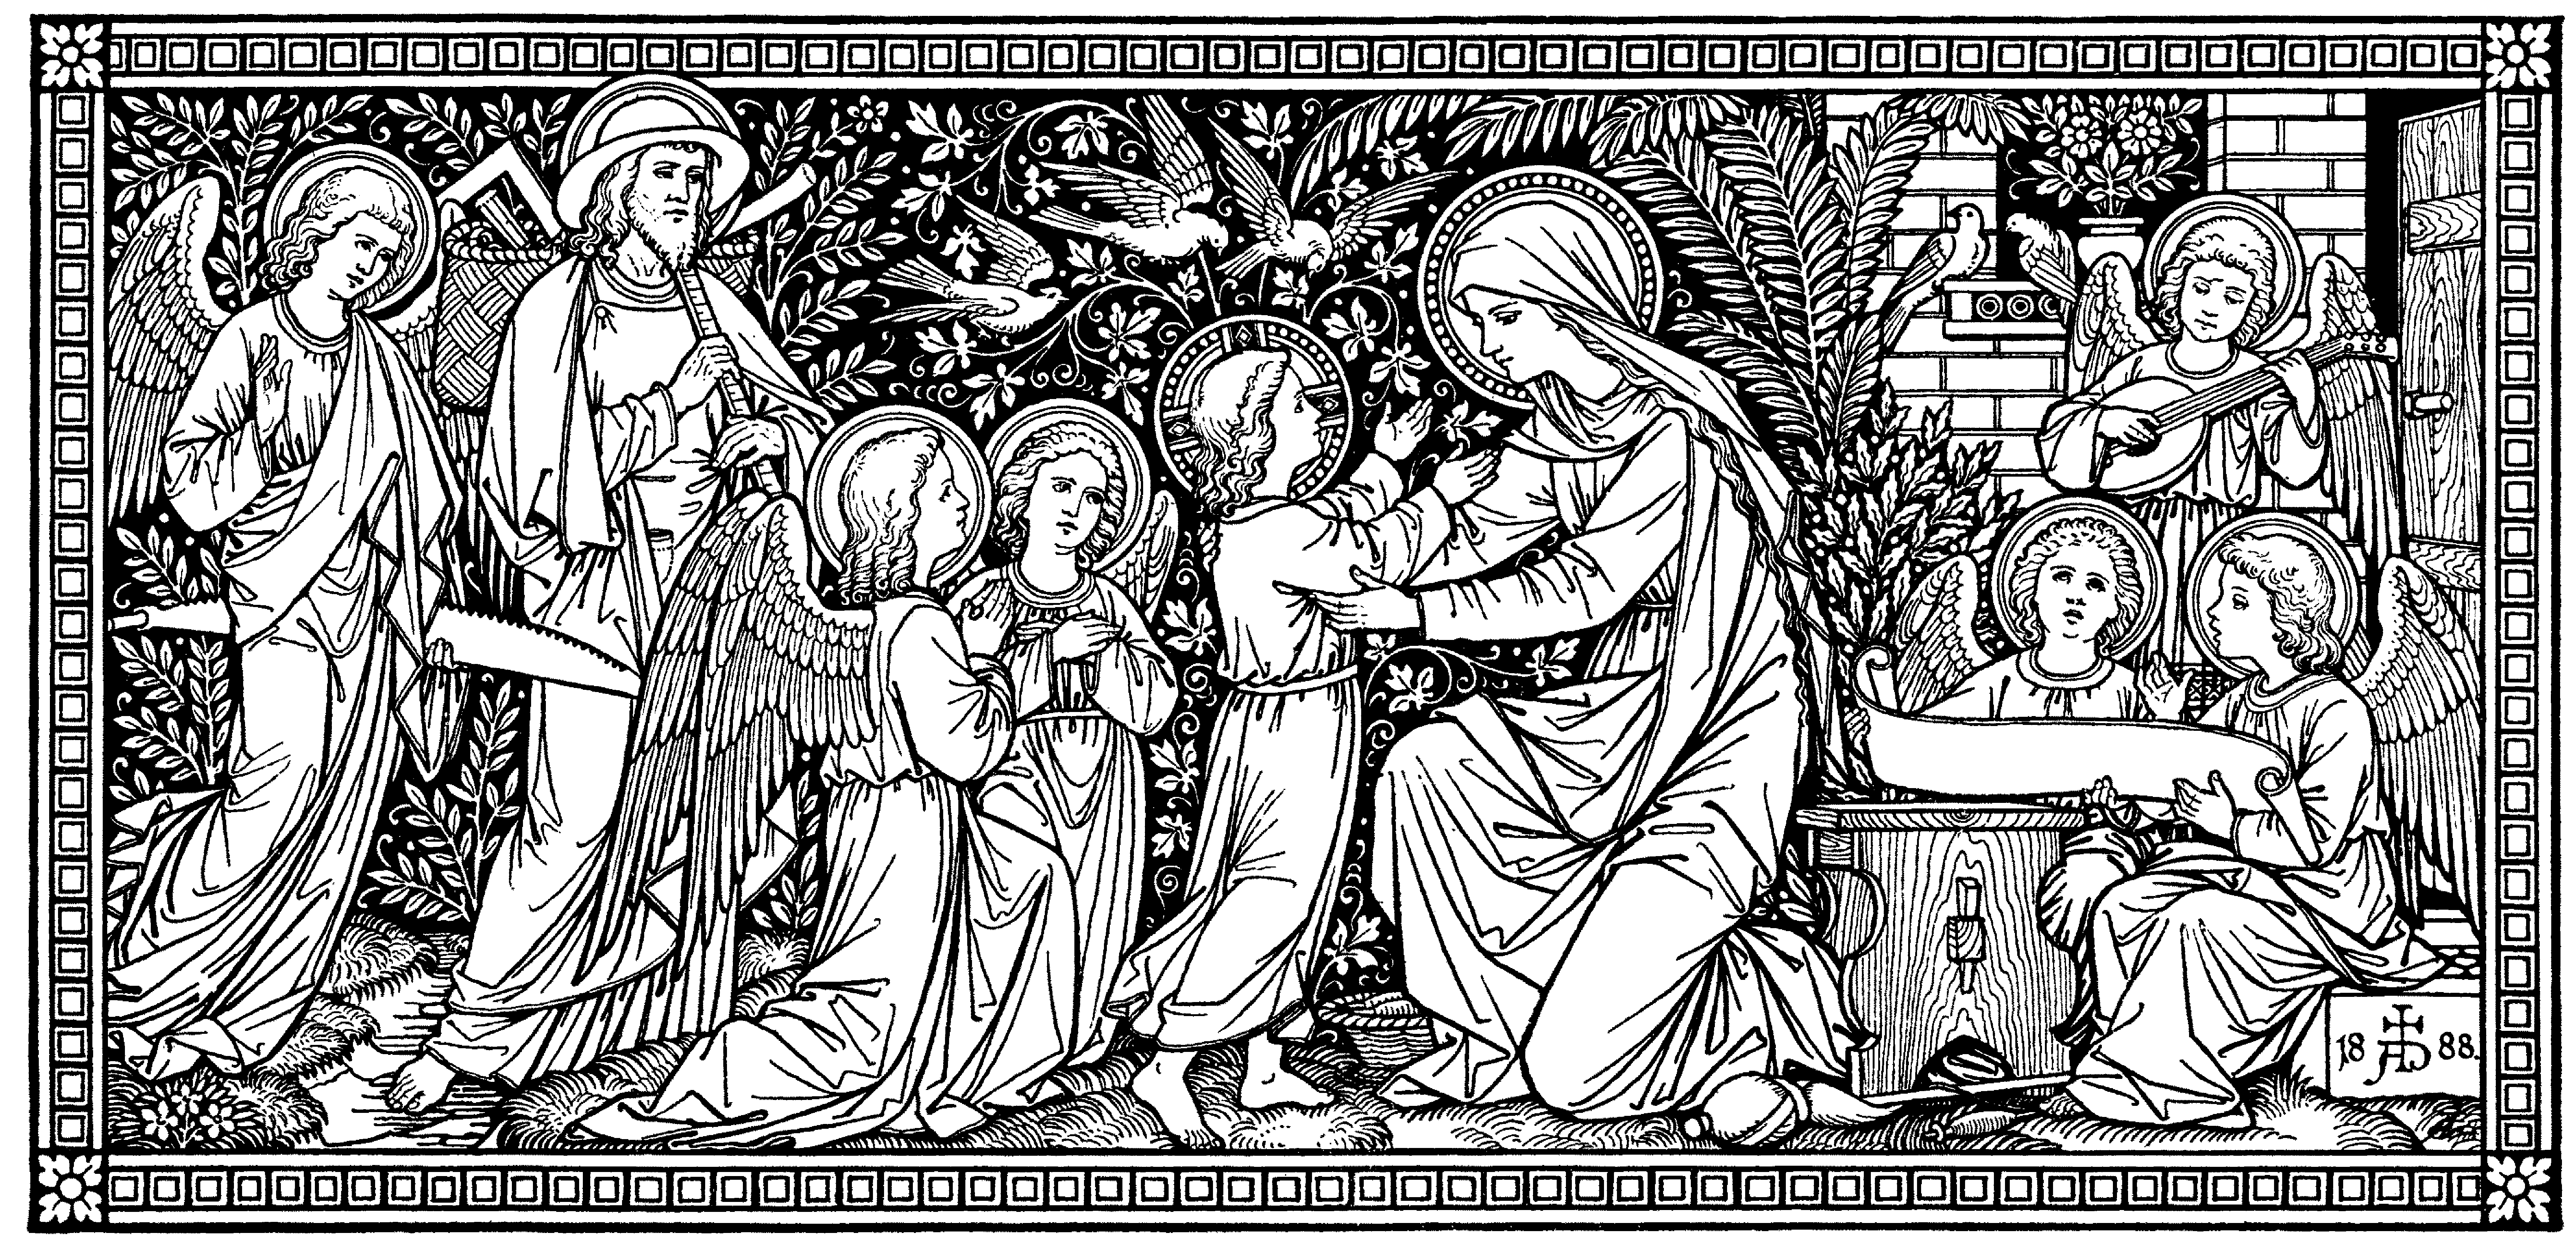
\includegraphics[height=5.5cm]{images/SainteFamille}
%\end{center}





\end{document}